%%% part-4.tex

\documentclass{standalone}

\usepackage{tikz}
\usetikzlibrary{decorations.pathreplacing}

\definecolor{myBlue}{RGB}{15,158,213}
\definecolor{myPurple}{RGB}{160,43,147}
\definecolor{myOrange}{RGB}{233,113,50}

\begin{document}
	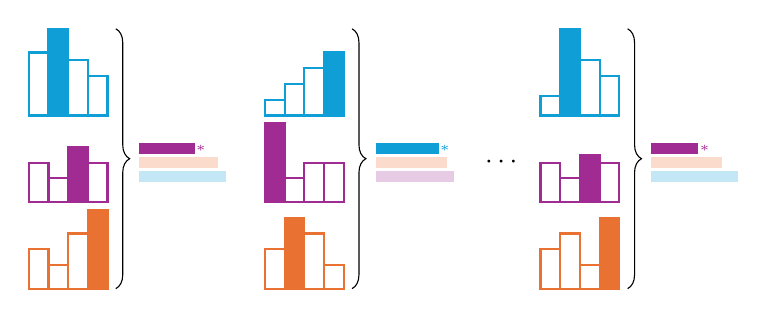
\begin{tikzpicture}
		\begin{scope}
			\begin{scope}[local bounding box=set1]
				\begin{scope}[yshift=1.1cm]
					\draw[myBlue,thick] (0,0) rectangle (0.25,0.8);
					\fill[myBlue,draw=myBlue,thick] (0.25,0) rectangle (0.5,1.1);
					\draw[myBlue,thick] (0.5,0) rectangle (0.75,0.7);
					\draw[myBlue,thick] (0.75,0) rectangle (1,0.5);
				\end{scope}
				\begin{scope}
					\draw[myPurple,thick] (0,0) rectangle (0.25,0.5);
					\draw[myPurple,thick] (0.25,0) rectangle (0.5,0.3);
					\fill[myPurple,draw=myPurple,thick] (0.5,0) rectangle (0.75,0.7);
					\draw[myPurple,thick] (0.75,0) rectangle (1,0.5);
				\end{scope}
				\begin{scope}[yshift=-1.1cm]
					\draw[myOrange,thick] (0,0) rectangle (0.25,0.5);
					\draw[myOrange,thick] (0.25,0) rectangle (0.5,0.3);
					\draw[myOrange,thick] (0.5,0) rectangle (0.75,0.7);
					\fill[myOrange,draw=myOrange,thick] (0.75,0) rectangle (1,1);
				\end{scope}
			\end{scope}
			\draw[decorate,decoration={brace,amplitude=5pt}] ([xshift=3pt]set1.north east) -- ([xshift=3pt]set1.south east) node[xshift=5pt,midway,right]{\tikz{\fill[myPurple] (0,3pt) rectangle (0.7,7pt) node[xshift=-3pt,yshift=-2.5pt,right]{\tiny *};\fill[myOrange!25] (0,2pt) rectangle (1,-2pt);\fill[myBlue!25] (0,-3pt) rectangle (1.1,-7pt);}};
		\end{scope}
		
		\begin{scope}[xshift=3cm]
			\begin{scope}[local bounding box=set2]
				\begin{scope}[yshift=1.1cm]
					\draw[myBlue,thick] (0,0) rectangle (0.25,0.2);
					\draw[myBlue,thick] (0.25,0) rectangle (0.5,0.4);
					\draw[myBlue,thick] (0.5,0) rectangle (0.75,0.6);
					\fill[white,thick] (0.75,0) rectangle (1,1.1);
					\fill[myBlue,draw=myBlue,thick] (0.75,0) rectangle (1,0.8);
				\end{scope}
				\begin{scope}
					\fill[myPurple,draw=myPurple,thick] (0,0) rectangle (0.25,1);
					\draw[myPurple,thick] (0.25,0) rectangle (0.5,0.3);
					\draw[myPurple,thick] (0.5,0) rectangle (0.75,0.5);
					\draw[myPurple,thick] (0.75,0) rectangle (1,0.5);
				\end{scope}
				\begin{scope}[yshift=-1.1cm]
					\draw[myOrange,thick] (0,0) rectangle (0.25,0.5);
					\fill[myOrange,draw=myOrange,thick] (0.25,0) rectangle (0.5,0.9);
					\draw[myOrange,thick] (0.5,0) rectangle (0.75,0.7);
					\draw[myOrange,thick] (0.75,0) rectangle (1,0.3);
				\end{scope}
			\end{scope}
			\draw[decorate,decoration={brace,amplitude=5pt}] ([xshift=3pt]set2.north east) -- ([xshift=3pt]set2.south east) node[xshift=5pt,midway,right]{\tikz{\fill[myBlue] (0,3pt) rectangle (0.8,7pt) node[xshift=-3pt,yshift=-2.5pt,right]{\tiny *};\fill[myOrange!25] (0,2pt) rectangle (0.9,-2pt);\fill[myPurple!25] (0,-3pt) rectangle (1,-7pt);}};
		\end{scope}
		
		\node at (6cm,0.5){$\cdots$};
		
		\begin{scope}[xshift=6.5cm]
			\begin{scope}[local bounding box=set3]
				\begin{scope}[yshift=1.1cm]
					\draw[myBlue,thick] (0,0) rectangle (0.25,0.25);
					\fill[myBlue,draw=myBlue,thick] (0.25,0) rectangle (0.5,1.1);
					\draw[myBlue,thick] (0.5,0) rectangle (0.75,0.7);
					\draw[myBlue,thick] (0.75,0) rectangle (1,0.5);
				\end{scope}
				\begin{scope}
					\draw[myPurple,thick] (0,0) rectangle (0.25,0.5);
					\draw[myPurple,thick] (0.25,0) rectangle (0.5,0.3);
					\fill[myPurple,draw=myPurple,thick] (0.5,0) rectangle (0.75,0.6);
					\draw[myPurple,thick] (0.75,0) rectangle (1,0.5);
				\end{scope}
				\begin{scope}[yshift=-1.1cm]
					\draw[myOrange,thick] (0,0) rectangle (0.25,0.5);
					\draw[myOrange,thick] (0.25,0) rectangle (0.5,0.7);
					\draw[myOrange,thick] (0.5,0) rectangle (0.75,0.3);
					\fill[myOrange,draw=myOrange,thick] (0.75,0) rectangle (1,0.9);
				\end{scope}
			\end{scope}
			\draw[decorate,decoration={brace,amplitude=5pt}] ([xshift=3pt]set3.north east) -- ([xshift=3pt]set3.south east) node[xshift=5pt,midway,right]{\tikz{\fill[myPurple] (0,3pt) rectangle (0.6,7pt) node[xshift=-3pt,yshift=-2.5pt,right]{\tiny *};\fill[myOrange!25] (0,2pt) rectangle (0.9,-2pt);\fill[myBlue!25] (0,-3pt) rectangle (1.1,-7pt);}};
		\end{scope}
	\end{tikzpicture}
\end{document}